\chapter{Sistema de normalización}
\label{ch:Normalizacion}

El circuito realizado para la linealización se basa en el formato IEEE 754, sin embargo el estimador de parámetros que se tiene, esta basado en un formato punto fijo, de manera que se debe considerar una conversión entre ambos formatos, para esto se estudió como pasar entre ambos formatos de punto flotante a punto fijo, ambos en 32-bits.


\section{Arquitectura}
\begin{figure}[H]
  \centering
    \includegraphics[scale=0.6]{./conversion_FF.png}
    \rule{35em}{0.5pt}
  \caption[conversión y normalización]{Proceso de conversión y normalización  }
  \label{fig:FF}
\end{figure}



  En la figura \ref{fig:FF} se puede observar el diagrama de solución que se utilizó para realizar la conversión, primeramente ingresa el numero en formato IEEE 754 32-bits, posteriormente se efectúa la conversión a punto fijo, en donde se asigna un bit de signo, 5 bits de parte entera y 26 bits para la parte fraccionaria, este dato se procesa en una etapa de normalización y se obtiene el resultado.
  
  \begin{figure}[H]
  \centering
    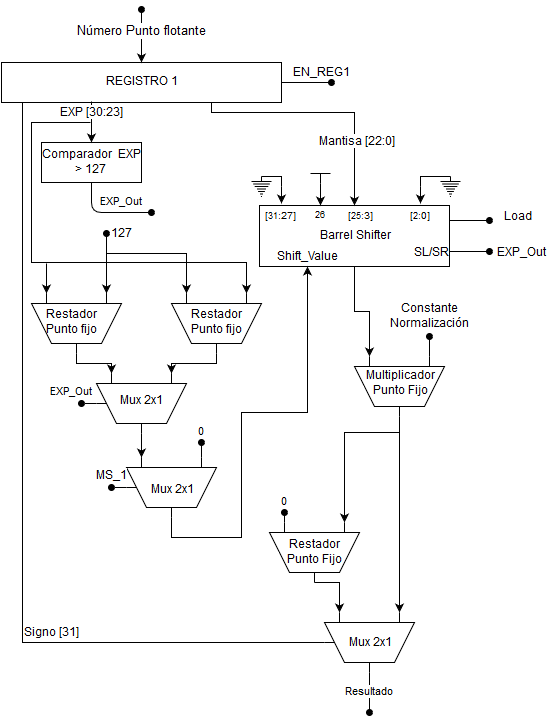
\includegraphics[scale=0.6]{./NORMALIZADOR.png}
    \rule{35em}{0.5pt}
  \caption[Normalizador]{Conversión punto flotante a punto fijo y normalización  }
  \label{fig:NORM}
\end{figure} 

Como se observa en la figura \ref{fig:NORM}, la etapa de conversión de formatos contiene un comparador, este se utiliza para saber si el numero contiene un exponente mayor o menor que 127, el numero 127 indica un exponente de 0, si es mayor la bandera de salida del comparador $\ EXP\_Out = 1$ , se debe realizar la operación $\ EXP - 127$, en caso contrario la bandera es 0 y la operación es $\ 127 - exp$, estas operaciones indican la cantidad de desplzamientos que se deben realizar en el Barrel shifter en donde la bandera $\ EXP\_Out $ indica la dirección de los desplazamientos. 

La etapa de normalización posee un multiplicador en punto fijo, las entradas de este contienen el valor convertido y una constante de normalización, esta constante se calcula en la siguiente ecuación: 
      

\begin{equation} \label{eq:ej1}
  C_{norm}
  = \frac{1}{Valor_{MAX}}  
\end{equation}  

La etapa de conversión y normalización se utiliza tanto para la corriente $\ i_{pv} $ como para la tensión $\ V_{pv} $ del panel, por lo tanto la constante de normalización varia para cada circuito,  
  
\begin{equation} \label{eq:ej2}
  Cv_{norm}
  = \frac{1}{18.1} = 0.055248618  
\end{equation}

\begin{equation} \label{eq:ej3}
  Ci_{norm}
  = \frac{1}{Ln\left(0.00667769\right)} = 0.199641045  
\end{equation}
 
 Donde $\ Cv_{norm}$ es la constante de normalización de la tensión y $\ Ci_{norm}$ la constante de normalización de la corriente. 
 
 Debido a que el resultado final de la conversión esta normalizado, $\ V = [0,1]$ e $\ i = [-1,1]$ para el formato punto fijo solo se requiere, un bit en la parte entera, como se muestra en la figura \ref{fig:FF} de manera que se pueden tomar mas bits para la parte fraccionaria y así obtener una mejor precisión en el resultado. 
 
\section{Control}

La arquitectura diseñada para el normalizador en su mayoría es combinacional sin embargo requiere un control, que detecta si se deben realizar  desplazamientos, y cuando se debe almacenar datos en registros. 

  \begin{figure}[H]
  \centering
    \includegraphics[scale=0.6]{./MaquinaFF.png}
    \rule{35em}{0.5pt}
  \caption[Control del normalizador]{Maquina de estados finita para el Normalizador}
  \label{fig:CTRLNORM}
\end{figure} 

El control de esta arquitectura se realiza por medio de una maquina de estado finita bastante sencilla, donde básicamente se cuenta con cuatro acciones principales, el primer estado (a) espera que sea iniciado mediante la señal $\ Begin\_FF$ y guarda el dato en el \nt{Registro 1}, el estado (b) verifica la condición $\ EXP=127 $ con esta se determina si se deben realizar desplazamientos, el estado (d) almacena en el Barrel-shifter el dato convertido, y en el estado (e) se indica mediante la bandera $\ ACK\_FF$ que el dato ya fue convertido y normalizado.

\section{Normalización en verilog}


\section{Simulación normalizador}

  \begin{figure}[H]
  \centering
    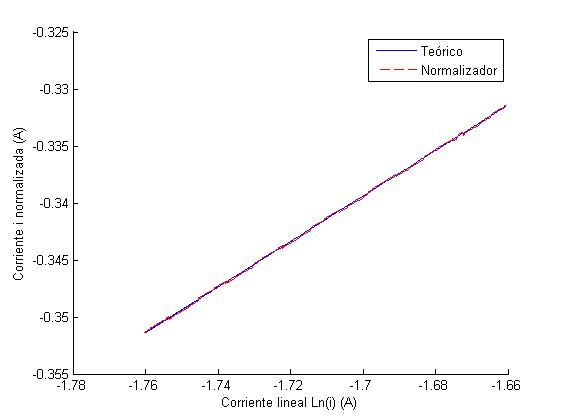
\includegraphics[scale=0.7]{./Normalizador_I.png}
    \rule{35em}{0.5pt}
  \caption[Normalizador de corriente]{Corriente $\ i_{pv}$ : Normalización teórica y normalización con circuito}
  \label{fig:NORMI}
\end{figure}

  \begin{figure}[H]
  \centering
    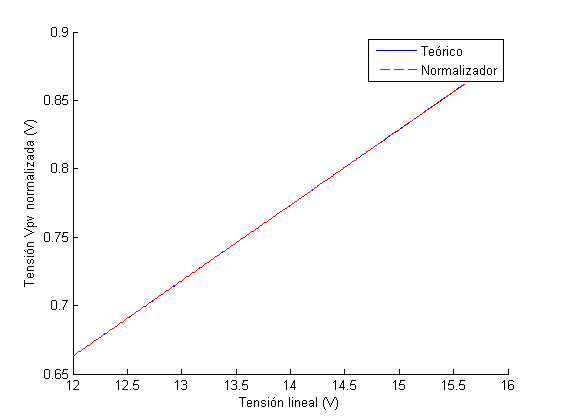
\includegraphics[scale=0.7]{./Normalizador_V.png}
    \rule{35em}{0.5pt}
  \caption[Normalizador de tensión]{Tensión $\ V_{pv}$ : Normalización teórica y normalización con circuito}
  \label{fig:NORMV}
\end{figure}
